\documentclass[a4paper]{article}
\usepackage[utf8]{inputenc}
\usepackage[english,russian]{babel}
\usepackage{indentfirst}
\usepackage{misccorr}
\usepackage{graphicx}
\graphicspath{{pics/}}
\usepackage{amsmath}
\usepackage[nottoc,numbib]{tocbibind}
\usepackage{multicol}
\usepackage{float}
\DeclareMathOperator*{\argmin}{arg\,min}
\usepackage[a4paper,margin=1.5cm]{geometry}
\usepackage{mathtools}
\DeclarePairedDelimiter\ceil{\lceil}{\rceil}

\usepackage{listings}
\usepackage{xcolor}
\begin{document}

\begin{titlepage}
    \thispagestyle{empty}

    \begin{center}
        \begin{figure}[htbp]
            \centering
            
\includegraphics[width=0.6\textwidth]{pics/msu.png}
        \end{figure}

        Московский Государственный Университет им. М.В. Ломоносова

        Факультет Вычислительной Математики и Кибернетики

        Кафедра Автоматизации Систем Вычислительных Комплексов

        \vfill
        \textbf{\huge Задание по курсу "Распределённые системы"}

        {\huge Отчёт}
    \end{center}

    \vfill
    \begin{flushright}
        {\large Выполнил:\\Попов Макар Сергеевич\\428 группа\\}
    \end{flushright}

    \centerline{Москва, 2022 год}

\end{titlepage}
\linespread{1.7}
\setcounter{page}{2}
\large

\tableofcontents
\newpage

\section{Постановка задач}

\subsection{Задание №1}
\textbf{Разработать программу которая реализует заданный алгоритм. Получить временную оценку работы алгоритма.}

В транспьютерной матрице размером 8*8, в каждом узле которой находится один процесс, необходимо выполнить операцию редукции MPI\_MAXLOC, определить глобальный максимум и соответствующих ему индексов. Каждый процесс предоставляет свое значение и свой номер в группе. Для всех процессов операция редукции должна возвратить значение максимума и номер первого процесса с этим значением.
Реализовать программу, моделирующую выполнение данной операции на транспьютерной матрице при помощи пересылок MPI типа точка-точка.
Оценить сколько времени потребуется для выполнения операции редукции, если все процессы выдали эту операцию редукции одновременно. Время старта равно 100, время передачи байта равно 1 (Ts=100,Tb=1). Процессорные операции, включая чтение из памяти и запись в память, считаются бесконечно быстрыми.

\subsection{Задание №2}

Доработать MPI-программу, реализованную в рамках курса “Суперкомпьютеры и параллельная обработка данных”. Добавить контрольные точки для продолжения работы программы в случае сбоя. Реализовать один из 3-х сценариев работы после сбоя: a) продолжить работу программы только на “исправных” процессах; б) вместо процессов, вышедших из строя, создать новые MPI-процессы, которые необходимо использовать для продолжения расчетов; в) при запуске программы на счет сразу запустить некоторое дополнительное количество MPI-процессов, которые использовать в случае сбоя.

\newpage

\section{Результаты}
\subsection{Задание №1}

Поскольку в условии задачи не указано число байт области памяти, подвергаемой редукции, будет считать, что оценка времени работы является функцией от длины этой области памяти. 

Операцию MPI\_MAXLOC разделим на два этапа: 
\begin{enumerate}
    \item редукцию значения с сохранением результата в корневом процессе
    \item рассылка значения от корневого процесса остальным
\end{enumerate}

Каждый из этапов операции выполняется посредством блокирующих операций получения и отправки сообщений MPI\_Recv и MPI\_Send.

Дабы минимизировать затраты времени, обусловленные временем старта передачи, представим транспьютерную матрицу в виде дерева (на примере 8-ми процессов):

\begin{figure}[htbp]
    \centering
    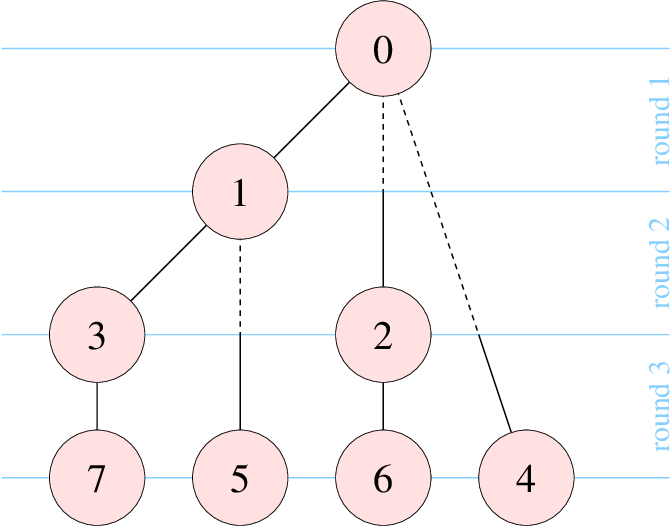
\includegraphics[width=0.6\textwidth]{pics/tree.png}
\end{figure}

Согласно представленной схеме отправки сообщений, на каждом этапе рассылаемая информация отправляется всеми процессами, которые уже ее получили. Для транспьютерной матрицы размера 8*8 потребуется $\log_2(64) =$ 6 этапов рассылки значения от корневого процесса остальным.

\newpage

Редукция значения происходит по той же схеме, но в противоположном направлении, что дает такую же оценку числа этапов пересылки.

Т.о. для области памяти размером n байт и p процессов время выполнения операции MPI\_MAXLOC равно:

$$ T(n) = T_s * (\ceil*{\log_2(p)} + T_b * n) $$

В случае $T_s = 100, T_b = 1, p = 64$:

$$ T(n) = 600 + 6n $$.

\newpage

\subsection{Задание №2}

MPI-программа, реализованная в рамках курса “Суперкомпьютеры и параллельная обработка данных”, представляет из себя параллельную версию метода Якоби, применяемого над 3-ехмерной матрицей.

Параллельность достигается за счет разделения исходной матрицы на непересекающиеся слои, выделяемые каждому рабочему процессу. В конце каждой итерации требуется синхронизация границ соседних слоев.

В рамках этой работы был реализован сценарий обработки сбоев, согласно которому в начале работы программы сразу запускается некоторое количество дополнительных MPI-процессов, которые используются в случае сбоя.

Принцип работы модифицированной программы состоит в следующем - при запуске всем доступным процессам назначается своя роль: \textit{процесс-мастер}, \textit{рабочий процесс} или \textit{восстановительный процесс}.

\subsubsection{Процесс-мастер}

Процесс-мастер (который бывает только в единственном экземпляре) отслеживает ход исполнения рабочих процессов.

В случае сбоя какого-либо из них, мастер отправляет запрос восстановительному процессу. Если восстановление прошло успешно, процесс-мастер сообщает соседям упавшего процесса ранг их нового соседа и исполнение возобновляется. Если восстановить процесс не удалось программа аварийно завершает работу.

В случае успешного завершения одного из рабочих процессов, процесс-мастер получает от него сообщение и далее не отслеживает ход исполнения этого процесса. Когда все рабочие процессы завершают работу, процесс-мастер должен принять данные о результате работы каждого из них и сохранить все слои полученной матрицы в своей памяти. Если к этому моменту остался хоть один восстанавливающий процесс, процесс-мастер отправит ему запрос на завершение.

\subsubsection{Рабочий процесс}

Рабочий процесс выполняет итерационные преобразования над выделенным слоем матрицы и проводит синхронизацию границ своего слоя с соседними процессами в конце каждой итерации. Если в каком-то из рабочих процессов произошел сбой, об этом узнает соседний процесс и передаст запрос на восстановление соседа процессу-мастеру, в ответ на отправленный запрос, мастер отправит ранг восстановленного соседа. Порядок синхронизации с соседями определяется в момент создания рабочего процесса.

Итерацию алгоритма, выполняемого рабочим процессом можно разделить на три этапа:

\begin{itemize}
    \item вычисление
    \item синхронизация с первым соседом (если таковой есть)
    \item синхронизация со вторым соседом (если таковой есть)
\end{itemize}

В конце каждого из этапов рабочий процесс создает контрольную точку, начиная с которой исполнение может быть возобновлено в случае сбоя. 

После всех итераций алгоритма рабочий процесс должен отправить свой слой матрицы процессу-мастеру и завершить работу.

\subsubsection{Восстанавливающий процесс}

Наконец, восстанавливающий процесс в начале работы встает на ожидание запроса от процесса-мастера. Если в поступившем запросе указан валидный ранг процесса, то восстанавливающий процесс пытается загрузить контрольную точку упавшего процесса. В случае успеха, восстанавливающий процесс оповещает процесс-мастер и входит в рабочий цикл рабочего процесса.

Если в поступившем от процесса-мастера запросе указан невалидный ранг, это означает, что все рабочие процессы успешно завершили работу, и восстанавливающий процесс поступает также.

\newpage

\section{Исходный код}

Весь исходный код программ приведен ниже, но также доступен в репозитории \url{https://github.com/SegFaulti4/distributed-systems} вместе с командами для запуска реализованных программ.

\lstdefinestyle{mystyle}{
    breakatwhitespace=false,         
    breaklines=true,
    keywordstyle=\bfseries\color{blue!50!black},
    commentstyle=\bfseries\color{green!35!black},
    stringstyle=\bfseries\color{red!50!black},
    basicstyle=\rmfamily\footnotesize,
    captionpos=b,                    
    keepspaces=true,                 
    numbers=left,                    
    numbersep=5pt,                  
    showspaces=false,                
    showstringspaces=false,
    showtabs=false,                  
    tabsize=2,
    frame = single
}

\lstset{style=mystyle}

\subsection{Задание №1}

\begin{lstlisting}[caption=transputer\_matrix.c, label={lst:1}, language=C]

#include <stdio.h>
#include <stdlib.h>
#include <mpi.h>
#include <string.h>

#define N_ROWS 8
#define N_COLS 8
#define NULL_RANK (-1)

#define Min(a,b) ((a)<(b)?(a):(b))
#define Max(a,b) ((a)>(b)?(a):(b))

int size = N_ROWS * N_COLS;
int rank;

// https://stackoverflow.com/a/15327567
int ceil_log2(unsigned long long x) {
    static const unsigned long long t[6] = {
        0xFFFFFFFF00000000ull,
        0x00000000FFFF0000ull,
        0x000000000000FF00ull,
        0x00000000000000F0ull,
        0x000000000000000Cull,
        0x0000000000000002ull
    };

    int y = (((x & (x - 1)) == 0) ? 0 : 1);
    int j = 32;
    int i;

    for (i = 0; i < 6; i++) {
        int k = (((x & t[i]) == 0) ? 0 : j);
        y += k;
        x >>= k;
        j >>= 1;
    }

    return y;
}

void init_binomial_heap(int *parent, int *children_num, int **children, int null_parent) {
    for (int i = 0; i < size; i++) {
        parent[i] = null_parent;
    }

    int *queue = calloc(size, sizeof(*queue));
    int *next_queue = calloc(size, sizeof(*next_queue));
    int depth = ceil_log2(size);
    children_num[0] = depth;
    children[0] = malloc(sizeof(**children) * children_num[0]);
    queue[0] = children_num[0];

    int next = 1;
    int reserved = children_num[0];
    int step = 1;

#ifdef DEBUG
    if (rank == 0) { printf("Sequence of messages during broadcast:\n"); }
#endif
    while (reserved) {
        memcpy(next_queue, queue, size * sizeof(*queue));
#ifdef DEBUG
        if (rank == 0) { printf("step %d: ", step); }
#endif
        for (int i = 0; i < size; i++) {
            if (queue[i] > 0) {
                children[i][children_num[i] - next_queue[i]] = next;
                parent[next] = i;
                next_queue[i]--;
#ifdef DEBUG
                if (rank == 0) { printf("%d -> %d ", i, next); }
#endif
                int child_count = Max(Min(size - next - reserved, next_queue[i]), 0);
                if (child_count == 0) {
                    children[next] = NULL;
                } else {
                    children[next] = malloc(sizeof(**children) * child_count);
                    next_queue[next] = child_count;
                    reserved += child_count;
                }
                children_num[next] = child_count;
                next++;
                reserved--;
            }
        }
#ifdef DEBUG
        if (rank == 0) { printf("\n"); }
#endif
        memcpy(queue, next_queue, size * sizeof(*queue));
        step++;
    }

    free(next_queue);
    free(queue);
}

void reduce_with_max(int *data, int *best_rank, MPI_Comm comm, int parent, int children_num, int *children) {
    if (children_num != 0) {
        int tmp;
        int other_rank;
        for (int i = 0; i < children_num; i++) {
            MPI_Recv(&tmp, 1, MPI_INT, children[i], 0, comm, MPI_STATUS_IGNORE);
            MPI_Recv(&other_rank, 1, MPI_INT, children[i], 0, comm, MPI_STATUS_IGNORE);
            if (tmp > *data) {
                *data = tmp;
                *best_rank = other_rank;
            }
        }
    }
    if (parent != NULL_RANK) {
        MPI_Send(data, 1, MPI_INT, parent, 0, comm);
        MPI_Send(best_rank, 1, MPI_INT, parent, 0, comm);
    }
}

void broadcast_data(int *data, int *best_rank, MPI_Comm comm, int parent, int children_num, int *children) {
    if (parent != NULL_RANK) {
        MPI_Recv(data, 1, MPI_INT, parent, 0, comm, MPI_STATUS_IGNORE);
        MPI_Recv(best_rank, 1, MPI_INT, parent, 0, comm, MPI_STATUS_IGNORE);
    }
    if (children_num != 0) {
        for (int i = 0; i < children_num; i++) {
            MPI_Send(data, 1, MPI_INT, children[i], 0, comm);
            MPI_Send(best_rank, 1, MPI_INT, children[i], 0, comm);
        }
    }
}

int main(int argc, char *argv[]) {
    MPI_Init(&argc, &argv);
    MPI_Comm_rank(MPI_COMM_WORLD, &rank);

    int *parent_rank = malloc(sizeof(*parent_rank) * size);
    int *children_num_rank = malloc(sizeof(*children_num_rank) * size);
    int **children_rank = malloc(sizeof(*children_rank) * size);
    init_binomial_heap(parent_rank, children_num_rank, children_rank, NULL_RANK);

    MPI_Comm comm;
    int dims[2] = {N_ROWS, N_COLS};
    int periods[2] = {0};
    int coords[2];

    MPI_Cart_create(MPI_COMM_WORLD, 2, dims, periods, 0, &comm);
    MPI_Cart_coords(comm, rank, 2, coords);

    int parent = parent_rank[rank];
    int children_num = children_num_rank[rank];
    int *children = children_rank[rank];

    srand(rank);
    int data = rand() % 1000000;
    int best_rank = rank;

    if (rank == 0) { printf("Generated data:\n"); }
    MPI_Barrier(comm);

    for (int i = 0; i < size; i++) {
        if (i == rank) {
            printf("rank: %d \tcoords: %d, %d\tdata: %d\n", rank, coords[0], coords[1], data);
            fflush(stdout);
        }
        MPI_Barrier(MPI_COMM_WORLD);
    }

    reduce_with_max(&data, &best_rank, comm, parent, children_num, children);
    MPI_Barrier(comm);
    if (rank == 0) { printf("\nMax data value: %d\nMax data rank: %d\n", data, best_rank); }

    broadcast_data(&data, &best_rank, comm, parent, children_num, children);
    int best_coords[2];
    MPI_Cart_coords(comm, best_rank, 2, best_coords);
    if (rank == 0) { printf("\nData after broadcast:\n"); }
    MPI_Barrier(comm);

    for (int i = 0; i < size; i++) {
        if (i == rank) {
            printf("rank: %d \tbest rank: %d\tbest coords: %d, %d\tdata: %d\n",
                   rank, best_rank, best_coords[0], best_coords[1], data);
            fflush(stdout);
        }
        MPI_Barrier(MPI_COMM_WORLD);
    }

    for (int i = 0; i < size; i++) {
        if (children_num_rank[i] != 0) {
            free(children_rank[i]);
        }
    }
    free(children_rank);
    free(children_num_rank);
    free(parent_rank);

    MPI_Finalize();
    return 0;
}

\end{lstlisting}

\newpage

\subsection{Задание №2: модифицированная версия}

\begin{lstlisting}[caption=jac\_3d\_mpi\_ft.c, label={lst:2}, language=C]

#include <math.h>
#include <stdlib.h>
#include <stdio.h>
#include <mpi.h>
#include <signal.h>
#include <unistd.h>

#define DEBUG 1
#define RECOVERY_PROC_NUM 1
#define NULL_RANK (-1)
#define NULL_WORKER (-1)
#define RECOVERY_IMPOSSIBLE 1
#define RECOVERY_FAILED 2

#define FIRST_SYNC_TAG 1215
#define SECOND_SYNC_TAG 1216
#define RECOVERY_REQ_TAG 1217
#define WORKER_FINISH_TAG 1218

#define N 34
#define MAX_ITERATIONS 100

#define Max(a,b) ((a)>(b)?(a):(b))
#define debug_m_printf if (DEBUG && !rank) printf
#define debug_printf if (DEBUG) printf

#define suicide if (rank == 1 && it_num == 2 && state == PENDING_FIRST_SYNC) { printf("Goodbye...\n"); fflush(stdout); raise(SIGTERM); }

/*
 * PROCESS ENTRY FUNCTIONS
 */

void master_entry();
void recovery_entry();
void worker_entry();

/*
 * WORKER PROCESS FUNCTIONS
 */

void worker_init();
void worker_state();
void worker_sync(int);
void free_workers_info();

/*
 * WORKER RECOVERY FUNCTIONS
 */

void save_worker_checkpoint();
void load_worker_checkpoint(int);
void worker_recovery(int, int);

/*
 * MATRIX OPERATION FUNCTIONS
 */

void matrix_init();
void compute();
void relax();
void resid();
void show_result();


// GENERAL INFO
int rank, size;
int recovery_proc_num, worker_proc_num;

// MASTER INFO
int *worker_rank, *worker_north_rank, *worker_south_rank, *worker_south_first;

// WORKER INFO
int north_rank, south_rank, south_first;
int start_row, last_row, it_num;

typedef enum {
    PENDING_COMPUTE,
    PENDING_FIRST_SYNC,
    PENDING_SECOND_SYNC
} Worker_state;

Worker_state state;

double A[N][N][N], B[N][N][N];
double eps;


int main(int argc, char **argv) {
    MPI_Init(&argc, &argv);
    MPI_Comm_rank(MPI_COMM_WORLD, &rank);
    MPI_Comm_size(MPI_COMM_WORLD, &size);

    recovery_proc_num = RECOVERY_PROC_NUM;
    worker_proc_num = size - 1 - recovery_proc_num;
    debug_m_printf("size: %d, recovery processes: %d, worker processes: %d\n", size, recovery_proc_num, worker_proc_num);

    if (worker_proc_num < 1) {
        debug_m_printf("Not enough worker processes - %d\n", worker_proc_num);
        MPI_Finalize();
        return 0;
    }

    worker_rank = malloc(sizeof(*worker_rank) * worker_proc_num);
    worker_north_rank = malloc(sizeof(*worker_north_rank) * worker_proc_num);
    worker_south_rank = malloc(sizeof(*worker_south_rank) * worker_proc_num);
    worker_south_first = malloc(sizeof(*worker_south_first) * worker_proc_num);

    for (int i = 0; i < worker_proc_num; i++) {
        int worker_r = i + 1;
        worker_rank[i] = worker_r;
        worker_north_rank[i] = worker_r == 1 ? NULL_RANK : worker_r - 1;
        worker_south_rank[i] = worker_r == worker_proc_num ? NULL_RANK : worker_r + 1;
        worker_south_first[i] = worker_r & 1;
        debug_m_printf("worker num: %d, rank: %d, north: %d, south: %d, south_first: %d\n",
                       i, worker_r, worker_north_rank[i], worker_south_rank[i], worker_south_first[i]);
    }

    MPI_Comm_set_errhandler(MPI_COMM_WORLD, MPI_ERRORS_RETURN);
    MPI_Barrier(MPI_COMM_WORLD);

    if (rank == 0) {
        master_entry();
    } else if (rank > worker_proc_num) {
        recovery_entry();
    } else {
        worker_entry();
    }

    MPI_Finalize();
    return 0;
}


/***************************
 * PROCESS ENTRY FUNCTIONS *
 ***************************/

void master_entry() {
    int unfinished_workers = worker_proc_num;
    int test[worker_proc_num];
    MPI_Request test_request[worker_proc_num];
    MPI_Status test_status;

    // Non-blocking receives from all workers
    for (int i = 0; i < worker_proc_num; i++) {
        MPI_Irecv(&test[i], 1, MPI_INT, worker_rank[i], WORKER_FINISH_TAG, MPI_COMM_WORLD, &test_request[i]);
    }

    while (unfinished_workers) {
        debug_printf("From %d (master) - unfinished workers: %d\n", rank, unfinished_workers);
        int idx = -1;

        // This operation completes if any worker is dead or finished
        MPI_Waitany(worker_proc_num, test_request, &idx, &test_status);
        debug_printf("From %d (master) - got message from %d: SOURCE: %d, TAG: %d, ERROR: %d\n",
                     rank, worker_rank[idx], test_status.MPI_SOURCE, test_status.MPI_TAG, test_status.MPI_ERROR);

        if (test_status.MPI_SOURCE != worker_rank[idx]) {
            // Found dead worker - try to recover
            int dead_rank = worker_rank[idx];
            debug_printf("From %d (master) - found dead process %d\n", rank, dead_rank);

            if (recovery_proc_num == 0) {
                printf("From %d (master) - no recovery processes, abort", rank);
                MPI_Abort(MPI_COMM_WORLD, RECOVERY_IMPOSSIBLE);
                return;
            }

            int recovery_proc_rank = size - recovery_proc_num;
            debug_printf("From %d (master) - recovering dead process with %d\n", rank, recovery_proc_rank);
            worker_rank[idx] = recovery_proc_rank;

            debug_printf("From %d (master) - sending recovery data to %d\n", rank, recovery_proc_rank);
            int err, tmp;
            MPI_Status tmp_status;
            err = MPI_Send(&dead_rank, 1, MPI_INT, recovery_proc_rank, RECOVERY_REQ_TAG, MPI_COMM_WORLD);
            if (!err) err = MPI_Send(&worker_north_rank[idx], 1, MPI_INT, recovery_proc_rank, RECOVERY_REQ_TAG, MPI_COMM_WORLD);
            if (!err) err = MPI_Send(&worker_south_rank[idx], 1, MPI_INT, recovery_proc_rank, RECOVERY_REQ_TAG, MPI_COMM_WORLD);
            if (!err) err = MPI_Send(&worker_south_first[idx], 1, MPI_INT, recovery_proc_rank, RECOVERY_REQ_TAG, MPI_COMM_WORLD);
            if (!err) err = MPI_Recv(&tmp, 1, MPI_INT, recovery_proc_rank, RECOVERY_REQ_TAG, MPI_COMM_WORLD, &tmp_status);

            if (err) {
                printf("From %d (master) - failed to recover process\n", rank);
                MPI_Abort(MPI_COMM_WORLD, RECOVERY_FAILED);
                return;
            }
            recovery_proc_num--;
            debug_printf("From %d (master) - successful recovery\n", rank);

            MPI_Request send_req[2];
            MPI_Status send_status[2];
            int count = 0;

            // Send recovered process rank to neighbours
            debug_printf("From %d (master) - sending data to %d and %d\n",
                         rank, worker_north_rank[idx], worker_south_rank[idx]);
            if (worker_north_rank[idx] != NULL_WORKER) {
                MPI_Isend(&recovery_proc_rank, 1, MPI_INT, worker_north_rank[idx], RECOVERY_REQ_TAG, MPI_COMM_WORLD, &send_req[count]);
                worker_south_rank[worker_north_rank[idx]] = recovery_proc_rank;
                count++;
            }
            if (worker_south_rank[idx] != NULL_WORKER) {
                MPI_Isend(&recovery_proc_rank, 1, MPI_INT, worker_south_rank[idx], RECOVERY_REQ_TAG, MPI_COMM_WORLD, &send_req[count]);
                worker_north_rank[worker_south_rank[idx]] = recovery_proc_rank;
                count++;
            }

            // Wait for neighbours to receive recovered process rank
            MPI_Waitall(count, send_req, send_status);
            if ((count >= 1 && send_status[0].MPI_ERROR) || (count >= 2 && send_status[1].MPI_ERROR)) {
                printf("From %d (master) - failed to send recovered rank\n", rank);
                MPI_Abort(MPI_COMM_WORLD, RECOVERY_FAILED);
                return;
            }
            debug_printf("From %d (master) - finished sending\n", rank);

            // Non-blocking receive from new process
            MPI_Irecv(&test[idx], 1, MPI_INT, worker_rank[idx], WORKER_FINISH_TAG, MPI_COMM_WORLD, &test_request[idx]);
        } else {
            // Process is not dead - it finished computing and now is waiting to send its data
            printf("From %d (master) - found finished process %d\n", rank, worker_rank[idx]);
            unfinished_workers--;
        }
    }
    debug_printf("From %d (master) - all workers finished\n", rank);

    debug_printf("From %d (master) - stopping recovery processes\n", rank);
    for (int i = 1; i <= recovery_proc_num; i++) {
        int tmp = NULL_RANK;
        debug_printf("From %d (master) - stop recovery proc %d\n", rank, size - i);
        MPI_Send(&tmp, 1, MPI_INT, size - i, RECOVERY_REQ_TAG, MPI_COMM_WORLD);
    }

    debug_printf("From %d (master) - receiving data from workers\n", rank);
    eps = 0.;
    for (int i = 0; i < worker_proc_num; i++) {
        MPI_Status status;
        double local_eps;
        debug_printf("From %d (master) - receiving data from %d\n", rank, worker_rank[i]);
        MPI_Recv(&start_row, 1, MPI_INT, worker_rank[i], WORKER_FINISH_TAG, MPI_COMM_WORLD, &status);
        MPI_Recv(&last_row, 1, MPI_INT, worker_rank[i], WORKER_FINISH_TAG, MPI_COMM_WORLD, &status);
        MPI_Recv(&A[start_row][0][0], (last_row - start_row + 1) * N * N, MPI_DOUBLE, worker_rank[i], WORKER_FINISH_TAG, MPI_COMM_WORLD, &status);
        MPI_Recv(&local_eps, 1, MPI_DOUBLE, worker_rank[i], WORKER_FINISH_TAG, MPI_COMM_WORLD, &status);
        eps = Max(eps, local_eps);
        debug_printf("From %d (master) - received data\n", rank);
    }
    start_row = 0;
    last_row = N - 1;

    debug_printf("From %d (master) - finished\n", rank);
    show_result();
}

void recovery_entry() {
    MPI_Status status;
    int dead_rank;
    debug_printf("From %d (recovery) - waiting request\n", rank);
    MPI_Recv(&dead_rank, 1, MPI_INT, 0, RECOVERY_REQ_TAG, MPI_COMM_WORLD, &status);
    if (dead_rank == NULL_RANK) {
        debug_printf("From %d (recovery) - gracefully stopping\n", rank);
        return;
    }
    debug_printf("From %d (recovery) - got request to recover %d\n", rank, dead_rank);

    MPI_Recv(&north_rank, 1, MPI_INT, 0, RECOVERY_REQ_TAG, MPI_COMM_WORLD, &status);
    MPI_Recv(&south_rank, 1, MPI_INT, 0, RECOVERY_REQ_TAG, MPI_COMM_WORLD, &status);
    MPI_Recv(&south_first, 1, MPI_INT, 0, RECOVERY_REQ_TAG, MPI_COMM_WORLD, &status);
    debug_printf("From %d (recovery) - received recovery data: north: %d, south: %d, south first: %d\n",
                 rank, north_rank, south_rank, south_first);

    load_worker_checkpoint(dead_rank);

    debug_printf("From %d (recovery) - successful loading, ack to master\n", rank);
    int tmp;
    MPI_Send(&tmp, 1, MPI_INT, 0, RECOVERY_REQ_TAG, MPI_COMM_WORLD);

    debug_printf("From %d (recovery) - entering worker loop\n", rank);
    worker_state();
}

void worker_entry() {
    worker_init();
    save_worker_checkpoint();
    debug_printf("From %d (worker) - saved first checkpoint\n", rank);
    worker_state();
}


/****************************
 * WORKER PROCESS FUNCTIONS *
 ****************************/

void worker_init() {
    north_rank = worker_north_rank[rank - 1];
    south_rank = worker_south_rank[rank - 1];
    south_first = worker_south_first[rank - 1];

    free_workers_info();

    int num_rows = (N - 2) / worker_proc_num;
    start_row = num_rows * (rank - 1) + 1;
    last_row = start_row + num_rows - 1;
    last_row += rank == worker_proc_num ? (N - 2) % worker_proc_num : 0;

    it_num = 0;
    state = PENDING_COMPUTE;

    matrix_init();
    debug_printf("From %d (worker) - initialized, start row: %d, last_row: %d\n", rank, start_row, last_row);
}

void worker_state() {
    for (; it_num < MAX_ITERATIONS; it_num++) {
        debug_printf("From %d (worker) - it_num: %d, state: %d\n", rank, it_num, state);
        switch (state) {
            case PENDING_COMPUTE:
                suicide
                compute();
                state = PENDING_FIRST_SYNC;
                save_worker_checkpoint();
                debug_printf("From %d (worker) - saved checkpoint\n", rank);

            case PENDING_FIRST_SYNC:
                suicide
                worker_sync(1);
                state = PENDING_SECOND_SYNC;
                save_worker_checkpoint();
                debug_printf("From %d (worker) - saved checkpoint\n", rank);

            case PENDING_SECOND_SYNC:
                suicide
                worker_sync(0);
                state = PENDING_COMPUTE;
                save_worker_checkpoint();
                debug_printf("From %d (worker) - saved checkpoint\n", rank);
        }
    }

    int tmp;
    debug_printf("From %d (worker) - ack to master\n", rank);
    MPI_Send(&tmp, 1, MPI_INT, 0, WORKER_FINISH_TAG, MPI_COMM_WORLD);

    debug_printf("From %d (worker) - sending data to master\n", rank);
    MPI_Send(&start_row, 1, MPI_INT, 0, WORKER_FINISH_TAG, MPI_COMM_WORLD);
    MPI_Send(&last_row, 1, MPI_INT, 0, WORKER_FINISH_TAG, MPI_COMM_WORLD);
    MPI_Send(&A[start_row][0][0], (last_row - start_row + 1) * N * N, MPI_DOUBLE, 0, WORKER_FINISH_TAG, MPI_COMM_WORLD);
    MPI_Send(&eps, 1, MPI_DOUBLE, 0, WORKER_FINISH_TAG, MPI_COMM_WORLD);
    debug_printf("From %d (worker) - finished\n", rank);
}

void worker_sync(int first_sync) {
    while (1) {
        MPI_Status status;
        int dest = south_first == first_sync ? south_rank : north_rank;
        debug_printf("From %d (worker) - entering sync with %d\n", rank, dest);
        void *sendbuf = south_first == first_sync ? &A[last_row][0][0] : &A[start_row][0][0];
        void *recvbuf = south_first == first_sync ? &A[last_row + 1][0][0] : &A[start_row - 1][0][0];

        if (dest != NULL_RANK) {
            int err = MPI_Sendrecv(sendbuf, N * N, MPI_DOUBLE, dest, first_sync ? FIRST_SYNC_TAG : SECOND_SYNC_TAG,
                                   recvbuf, N * N, MPI_DOUBLE, dest, first_sync ? FIRST_SYNC_TAG : SECOND_SYNC_TAG, MPI_COMM_WORLD, &status);
            if (err) {
                printf("From %d (worker) - Process %d appears to be dead\n", rank, dest);
                worker_recovery(dest, south_first == first_sync);
                continue;
            }
            debug_printf("From %d (worker) - successful sync with %d\n", rank, dest);
        } 
        break;
    } 
}

void free_workers_info() {
    if (worker_rank)        free(worker_rank);
    if (worker_north_rank)  free(worker_north_rank);
    if (worker_south_rank)  free(worker_south_rank);
    if (worker_south_first) free(worker_south_first);

    worker_rank = NULL;
    worker_north_rank = NULL;
    worker_south_rank = NULL;
    worker_south_first = NULL;
}


/*****************************
 * WORKER RECOVERY FUNCTIONS *
 *****************************/

void save_worker_checkpoint() {
    debug_printf("From %d (worker) - saving checkpoint: it_num: %d, state: %d\n", rank, it_num, state);
    char path[100];
    snprintf(path, 100, "CP/control_point_%d.bin", rank);

    FILE *cp_file = fopen(path, "wb");

    if (cp_file == NULL) {
        printf("From %d (worker) - could not save checkpoint\n", rank);
        raise(SIGTERM);
        return;
    }

    fwrite(&start_row, sizeof(start_row), 1, cp_file);
    fwrite(&last_row, sizeof(last_row), 1, cp_file);
    fwrite(&it_num, sizeof(it_num), 1, cp_file);
    fwrite(&state, sizeof(state), 1, cp_file);
    fwrite(&eps, sizeof(eps), 1, cp_file);

    int start = north_rank == NULL_RANK ? start_row : start_row - 1;
    int end = south_rank == NULL_RANK ? last_row : last_row + 1;

    fwrite(&A[start][0][0], sizeof(double), (end - start + 1) * N * N, cp_file);

    fclose(cp_file);
    sync();
}

void load_worker_checkpoint(int dead) {
    debug_printf("From %d (recovery) - loading checkpoint of %d\n", rank, dead);
    char path[100];
    snprintf(path, 100, "CP/control_point_%d.bin", dead);

    sync();
    FILE *cp_file = fopen(path, "rb");

    if (cp_file == NULL) {
        printf("From %d (recovery) - could not load checkpoint\n", rank);
        raise(SIGTERM);
        return;
    }

    fread(&start_row, sizeof(start_row), 1, cp_file);
    fread(&last_row, sizeof(last_row), 1, cp_file);
    fread(&it_num, sizeof(it_num), 1, cp_file);
    fread(&state, sizeof(state), 1, cp_file);
    fread(&eps, sizeof(eps), 1, cp_file);

    int start = north_rank == NULL_RANK ? start_row : start_row - 1;
    int end = south_rank == NULL_RANK ? last_row : last_row + 1;

    fread(&A[start][0][0], sizeof(double), (end - start + 1) * N * N, cp_file);

    fclose(cp_file);
}

void worker_recovery(int dead, int south) {
    int err = MPI_Send(&dead, 1, MPI_INT, 0, RECOVERY_REQ_TAG, MPI_COMM_WORLD);
    if (err) {
        printf("From %d (worker) - failed to send recovery request\n", rank);
        MPI_Abort(MPI_COMM_WORLD, RECOVERY_FAILED);
        return;
    }
    MPI_Status status;
    MPI_Recv(south ? &south_rank : &north_rank, 1, MPI_INT, 0, RECOVERY_REQ_TAG, MPI_COMM_WORLD, &status);
}


/******************************
 * MATRIX OPERATION FUNCTIONS *
 ******************************/

void matrix_init() {
    for (int i = start_row - 1; i <= last_row + 1; i++) {
        for (int j = 0; j <= N - 1; j++) {
            for (int k = 0; k <= N - 1; k++) {
                if (i == 0 || i == N - 1 || j == 0 || j == N - 1 || k == 0 || k == N - 1) {
                    A[i][j][k] = 0.;
                } else {
                    A[i][j][k] = (4. + i + j + k);
                }
            }
        }
    }
}

void compute() {
    relax();
    resid();
}

void relax() {
    debug_printf("From %d (worker) - started relax\n", rank);
    for (int i = start_row; i <= last_row; i++) {
        for (int j = 1; j <= N - 2; j++) {
            for (int k = 1; k <= N - 2; k++) {
                B[i][j][k] = (A[i - 1][j][k] + A[i + 1][j][k] + A[i][j - 1][k] +
                              A[i][j + 1][k] + A[i][j][k - 1] + A[i][j][k + 1]) / 6.;
            }
        }
    }
}

void resid() {
    int start_flag = start_row == 0 ? 1 : 0;
    int last_flag = last_row == N - 1 ? 1 : 0;

    start_row = start_flag ? start_row + 1 : start_row;
    last_row = last_flag ? last_row - 1 : last_row;

    debug_printf("From %d (worker) - started resid\n", rank);
    eps = 0.;
    for (int i = start_row; i <= last_row; i++) {
        for (int j = 1; j <= N - 2; j++) {
            for (int k = 1; k <= N - 2; k++) {
                double e;
                e = fabs(A[i][j][k] - B[i][j][k]);
                A[i][j][k] = B[i][j][k];
                eps = Max(eps, e);
            }
        }
    }
    debug_printf("From %d (worker) - resid eps: %lf\n", rank, eps);

    start_row = start_flag ? start_row - 1 : start_row;
    last_row = last_flag ? last_row + 1 : last_row;
}

void show_result() {
    double s = 0.0;
    for (int i = start_row; i <= last_row; i++) {
        for (int j = 0; j <= N - 1; j++) {
            for (int k = 0; k <= N - 1; k++) {
                s = s + A[i][j][k] * (i + 1) * (j + 1) * (k + 1) / (N * N * N);
            }
        }
    }

    printf("S = %lf\neps = %lf\n", s, eps);

    FILE * res = fopen("result_ft.txt", "w");
    for (int i = start_row; i <= last_row; i++) {
        for (int j = 0; j <= N - 1; j++) {
            for (int k = 0; k <= N - 1; k++) {
                fprintf(res, "%lf ", A[i][j][k]);
            }
            fprintf(res, "\n");
        }
        fprintf(res, "\n");
    }
    fclose(res);
}

\end{lstlisting}

\newpage

\subsection{Задание №2: исходная версия}

\begin{lstlisting}[caption=jac\_3d\_mpi\_noft.c, label={lst:3}, language=C]

#include <math.h>
#include <stdio.h>
#include <mpi.h>

#define DEBUG 1

#define FIRST_SYNC_TAG 1215
#define SECOND_SYNC_TAG 1216
#define FINISH_TAG 1218

#define N 34
#define MAX_ITERATIONS 100

#define Max(a,b) ((a)>(b)?(a):(b))
#define debug_m_printf if (DEBUG && !rank) printf
#define debug_printf if (DEBUG) printf


void sync_edges();

void matrix_init();
void compute();
void relax();
void resid();
void show_result();


int rank, size;
int start_row, last_row;

double A[N][N][N], B[N][N][N];
double eps;


int main(int argc, char **argv) {
    MPI_Init(&argc, &argv);
    MPI_Comm_rank(MPI_COMM_WORLD, &rank);
    MPI_Comm_size(MPI_COMM_WORLD, &size);

    debug_m_printf("size: %d\n", size);

    int num_rows = (N - 2) / size;
    start_row = num_rows * rank + 1;
    last_row = start_row + num_rows - 1;
    last_row += (rank == size - 1) ? (N - 2) % size : 0;
    debug_printf("rank: %d, startrow: %d, lastrow: %d\n", rank, start_row, last_row);

    matrix_init();

    for (int it_num = 0; it_num < MAX_ITERATIONS; it_num++) {
        compute();
        sync_edges();
    }

    if (rank == 0) {
        debug_printf("Receiving data\n");
        MPI_Comm_size(MPI_COMM_WORLD, &size);
        for (int i = 1; i < size; i++) {
            MPI_Status status;
            double local_eps;
            MPI_Recv(&start_row, 1, MPI_INT, i, FINISH_TAG, MPI_COMM_WORLD, &status);
            MPI_Recv(&last_row, 1, MPI_INT, i, FINISH_TAG, MPI_COMM_WORLD, &status);
            MPI_Recv(&A[start_row][0][0], (last_row - start_row + 1) * N * N, MPI_DOUBLE, i, FINISH_TAG, MPI_COMM_WORLD, &status);
            MPI_Recv(&local_eps, 1, MPI_DOUBLE, i, FINISH_TAG, MPI_COMM_WORLD, &status);
            eps = Max(eps, local_eps);
        }
        start_row = 0;
        last_row = N - 1;

        MPI_Barrier(MPI_COMM_WORLD);
        debug_printf("Finished\n");
        show_result();
    } else {
        debug_printf("Sending data from %d\n", rank);
        MPI_Send(&start_row, 1, MPI_INT, 0, FINISH_TAG, MPI_COMM_WORLD);
        MPI_Send(&last_row, 1, MPI_INT, 0, FINISH_TAG, MPI_COMM_WORLD);
        MPI_Send(&A[start_row][0][0], (last_row - start_row + 1) * N * N, MPI_DOUBLE, 0, FINISH_TAG, MPI_COMM_WORLD);
        MPI_Send(&eps, 1, MPI_DOUBLE, 0, FINISH_TAG, MPI_COMM_WORLD);
        MPI_Barrier(MPI_COMM_WORLD);
    }

    MPI_Finalize();
    return 0;
}

void matrix_init() {
    for (int i = start_row - 1; i <= last_row + 1; i++) {
        for (int j = 0; j <= N - 1; j++) {
            for (int k = 0; k <= N - 1; k++) {
                if (i == 0 || i == N - 1 || j == 0 || j == N - 1 || k == 0 || k == N - 1) {
                    A[i][j][k] = 0.;
                } else {
                    A[i][j][k] = (4. + i + j + k);
                }
            }
        }
    }
}

void compute() {
    relax();
    resid();
}

void relax() {
    debug_m_printf("Started relax\n");
    for (int i = start_row; i <= last_row; i++) {
        for (int j = 1; j <= N - 2; j++) {
            for (int k = 1; k <= N - 2; k++) {
                B[i][j][k] = (A[i - 1][j][k] + A[i + 1][j][k] + A[i][j - 1][k] +
                              A[i][j + 1][k] + A[i][j][k - 1] + A[i][j][k + 1]) / 6.;
            }
        }
    }
}

void resid() {
    int start_flag = start_row == 0 ? 1 : 0;
    int last_flag = last_row == N - 1 ? 1 : 0;

    start_row = start_flag ? start_row + 1 : start_row;
    last_row = last_flag ? last_row - 1 : last_row;

    debug_m_printf("Started resid\n");
    eps = 0.;
    for (int i = start_row; i <= last_row; i++) {
        for (int j = 1; j <= N - 2; j++) {
            for (int k = 1; k <= N - 2; k++) {
                double e;
                e = fabs(A[i][j][k] - B[i][j][k]);
                A[i][j][k] = B[i][j][k];
                eps = Max(eps, e);
            }
        }
    }
    debug_m_printf("Resid eps: %lf\n", eps);

    start_row = start_flag ? start_row - 1 : start_row;
    last_row = last_flag ? last_row + 1 : last_row;
}

void show_result() {
    double s = 0.0;
    for (int i = start_row; i <= last_row; i++) {
        for (int j = 0; j <= N - 1; j++) {
            for (int k = 0; k <= N - 1; k++) {
                s = s + A[i][j][k] * (i + 1) * (j + 1) * (k + 1) / (N * N * N);
            }
        }
    }

    printf("S = %lf\neps = %lf\n", s, eps);

    FILE * res = fopen("result_noft.txt", "w");
    for (int i = start_row; i <= last_row; i++) {
        for (int j = 0; j <= N - 1; j++) {
            for (int k = 0; k <= N - 1; k++) {
                fprintf(res, "%lf ", A[i][j][k]);
            }
            fprintf(res, "\n");
        }
        fprintf(res, "\n");
    }
    fclose(res);
}

void sync_edges() {
    MPI_Request request[4];
    MPI_Status status[4];

    MPI_Comm_size(MPI_COMM_WORLD, &size);
    if (rank) {
        MPI_Irecv(&A[start_row - 1][0][0], N * N, MPI_DOUBLE, rank - 1, FIRST_SYNC_TAG, MPI_COMM_WORLD, &request[0]);
        MPI_Isend(&A[start_row][0][0], N * N, MPI_DOUBLE, rank - 1, SECOND_SYNC_TAG, MPI_COMM_WORLD, &request[1]);
    }
    if (rank != size - 1) {
        MPI_Isend(&A[last_row][0][0], N * N, MPI_DOUBLE, rank + 1, FIRST_SYNC_TAG, MPI_COMM_WORLD, &request[2]);
        MPI_Irecv(&A[last_row + 1][0][0], N * N, MPI_DOUBLE, rank + 1, SECOND_SYNC_TAG, MPI_COMM_WORLD, &request[3]);
    }

    int ll = 4, shift = 0;
    if (!rank) {
        ll -= 2;
        shift = 2;
    }
    if (rank == size - 1) {
        ll -= 2;
    }
    if (ll) {
        MPI_Waitall(ll, &request[shift], status);
    }
}

\end{lstlisting}
\end{document}

